\chapter{序論}

\section{はじめに}
1953年、James WatsonとFrancis Crickは、遺伝情報の実体は4種類のデオキリボ核酸が相補的に水素結合した二重らせん構造を持つことを分子模型を使い鮮やかに示した。5年後の
1958年、Clickは"Ideas for protein synthesis"において、遺伝情報はDNA-RNA-タンパクへと一方向性を持って伝達されるという分子生物学における中心原理をセントラルドグマとして提唱した (図 \ref{fig:crick_idea})。1960年代から70年代には、Maurice WilkinsやSydney Brennerなど多くの研究者によって、コドンの発見と遺伝暗号が解読され、塩基配列がアミノ酸を表現する基本原則が明らかにされてきた。黎明期における分子生物学は、当時の物理学者が多く参入した経緯も相まって、分子のことばで生命の持つ普遍的性質の理解を標榜する学問として誕生し、熾烈な競争の下に急速な発展を遂げた。
\begin{figure}[htbp]
	\begin{center}
		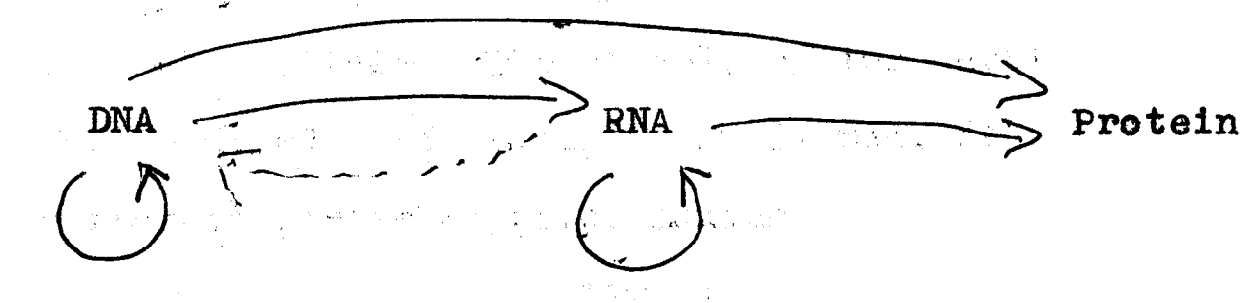
\includegraphics[width=14cm]{crick_idea.png}
	\end{center}
	\caption{"Ideas on Protein Synthesis", (Oct, 1956)}
	\label{fig:crick_idea}
\end{figure}
\par
今日までの分子生物学研究の進展は、普遍的だと考えられてきた数々の性質や分子機序からの逸脱や例外をも同時に明らかにしてきた。1970年、Howard TeminおよびDavid Baltimoreは一本鎖RNAをテンプレートとして、相補的なDNAを合成する逆転写酵素を発見した。この発見は、セントラルドグマから逸脱し、RNAからDNAへも遺伝情報は伝達しうることを示した画期的な発見であった。その後も、真核生物における遺伝子はスプライシング機構によってイントロンが切り出され複数のエクソンから構成されること、転写直後の新生RNAは3'末端にポリアデニル化、5'末端にはキャップ構造が付加されて成熟すること、コドンが異なるアミノ酸をコードする例外が発見され、セントラルドグマの概念もまた拡張されてきた。このことは、本質的には、生命が多様性を担保する存在であることに他ならないことを示している。生命が持つ普遍的な性質の理解を目指した分子生物学において、逸脱や例外といった個別的な生命現象をその対象することが逆説的には、生命の理解へと接続される重要なアプローチだと私は考えている。
%\par
%転写はゲノム上にコードされた遺伝情報をRNAへ正確にコピーする機構を指す。転写は核内で起こる生化学反応であり、RNAポリメラーゼよって触媒される。転写されたpre-mRNAはスプライシング、ポリアデニル化と5'キャップ付加を受けて成熟した後に、核膜孔を通して細胞質へ輸送される、というのが転写機構の大まかな素描である。ヒトゲノムの解読前、遺伝子数はおよそ10万個だと見積もられていたが、2004年の完了宣言では2.5万個程度に大きく下方修正され、直感的な生命の複雑性と遺伝子数には直接の相関関係が見られないことは今日に繰り返すまでもない。
\par
真核生物の多様で複雑なシステムは、セントラルドグマからの逸脱の他に塩基やタンパク質への修飾にその大部分を依存していることは前提となりつつある。細胞の内外の情報伝達には、キナーゼによるタンパク質のカスケード的なリン酸化反応が用いられ、リン酸化された分子が核内に移行し転写因子の活性を調節することで遺伝子発現の状態と量が制御される。ヒストンにおいては、アセチル基やメチル基による修飾を受け、染色体構造の変化を伴った遺伝子発現調節や細胞の分化状態が制御されるなど、修飾の持つ生体内機序の制御例は枚挙にいとまがない。真核生物においては有限個の遺伝子にその多様性を規定されながらも、転写・翻訳機構からの逸脱や修飾によって多様かつ複雑な制御機構が実現されている。
\par
本研究が対象としているのはRNA editing (RNA編集)という転写後修飾 (post-transcriptional modification)の一種である。RNA 
editingは、DNAにコードされた遺伝情報がRNAへ転写された直後、別の塩基に置換される現象を指す。RNA editingを受けた転写物は、元来の遺伝情報とは異なった塩基情報を持つこととなる。この塩基修飾は、DNAから正確なコピーとしてのRNAを合成するという転写機構からの明らかな逸脱と考えることができる。興味深いことにヒトやマウス、ショウジョウバエといった高等真核生物では遺伝子配列内へ積極的にRNA editingを起こし、異なる機能を有したタンパクを機能させている報告がある。ここ数年の超並列シーケンシング (High-throughput sequencing)によるトランスクリプトームの網羅的かつ定量的な計測は、non-coding RNAやイントロン領域などこれまで研究対象とされなかったゲノム領域におけるRNA editingに光を当てたことから、今日において非常に注目を集めている分野の一つである。
\par
本研究は、ゲノムワイドなRNA editingサイトの検出手法の開発とその情報学的解析を行ったものである。序論では、これまでのRNA editingの生理学的な機能、超並列シーケンサーを用いたRNA editing研究について概観する。第2章および3章では、既存の検出手法について性能評価を行い、高精度かつ高速な新規RNA editingサイトの検出手法の開発に関する研究を行った。第4章では、開発した手法をヨコヅナクマムシへ適用し、RNA editingと極限環境耐性との関係性についての情報学的解析を行った。本研究は、大量のRNA-seqデータを用いたRNA editingサイトの簡便な検出を可能にし、生命における普遍性からの逸脱や例外による制御・調節機構への解明に大きく貢献することを期待する。
\newpage

\section{真核生物におけるADARの作用機序}
\subsection{ADARによるA-to-I editing}
RNA editingは転写物への一塩基修飾を指し、鞭毛虫のミトコンドリアRNAから初めて発見された。真核生物では、アデニン(A)からイノシン(I)へ修飾されるA-to-I editingの他に、シトシン(C)からチミン(T)への修飾がこれまで報告されている。植物においてはT-to-C editing、ヒトやマウス、ショウジョウバエなど高等真核生物においてはA-to-I editingが優勢を占めることが多くの研究から明らかになっている。しかしながら、アミノ酸配列の変化を伴うA-to-I editingの報告例は非コード領域におけるeditingに対して著しく少なく、非翻訳領域 (Untranslated regions, UTRs)やAlu配列といったイントロン内のレトロトランスポゾン領域におけるA-to-I editingが優勢を占めていることが明らかになっている。加えて、miRNAやRNAi経路とのクロストークを介したグローバルな遺伝子発現制御との関係性などが指摘されていることから、真核生物におけるA-to-I editingを理解するためには、non-coding RNAにおけるA-to-I editingを研究することが極めて重要であると言える。すなわち、真核生物におけるRNA editingの理解には、従来想定されてきたようなアミノ酸置換を伴ったコード領域内へのeditingのみならず、非コード領域におけるeditingを研究し、その意味を理解することの重要性を示している。本論はこの視点に立脚し、RNA editing研究に関する最新の研究成果を含めて分野を概観すると同時に、今後のediting研究の進むであろう一つの方向性を示すことができればと考える。
\begin{figure}[htbp]
	\begin{center}
		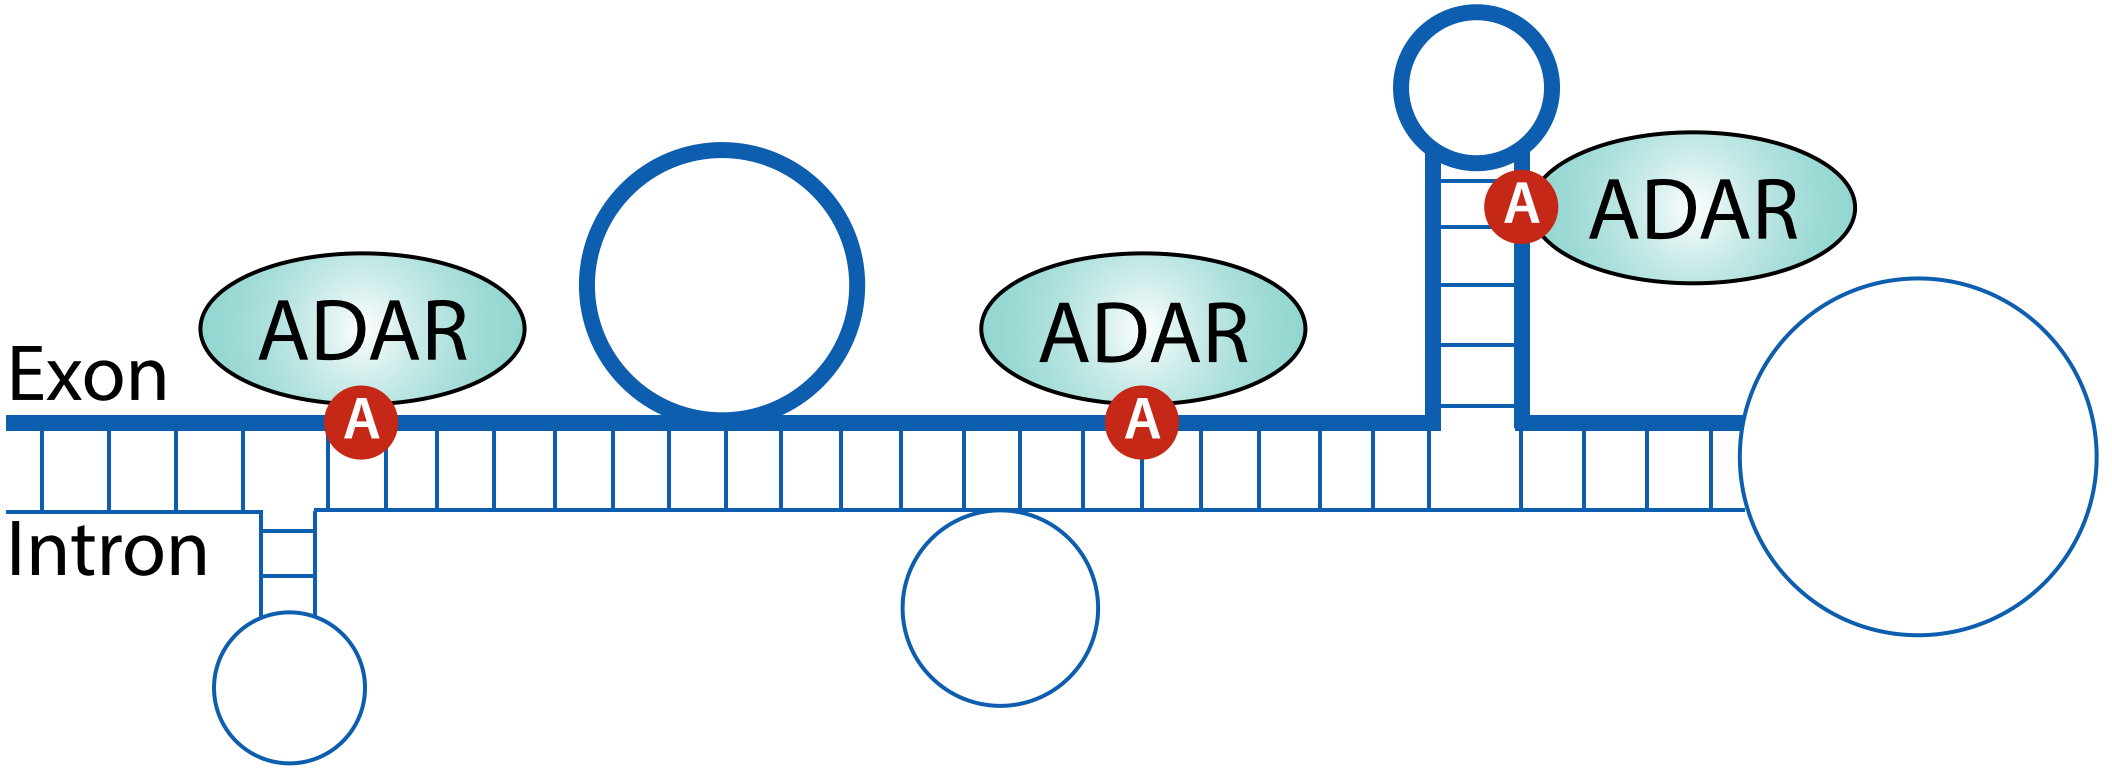
\includegraphics[width=14cm]{ADAR.png}
	\end{center}
	\caption{ADARによるA-to-I editingの模式図}
	\begin{flushleft}
		\small{ADARは二次構造を形成した二本鎖RNAへ結合し、A-to-I editingを触媒する。多くの転写物は一つ以上の複数のeditingサイトを持つ。この図では、エクソン領域(太線)と隣接するイントロン領域(細線)の間に二次構造が形成されている様子を表している。}
	\end{flushleft}
	\label{fig:ADAR}
\end{figure}

\subsection{ADARの作用機序}
ADAR (adenosine deaminase acting on RNA)は、二本鎖RNA結合タンパクの一種として知られ、二本鎖RNAと選択的に結合し、アデノシン (Adenosine)からイノシン (Inosine)への脱アミノ化反応を触媒する (A-to-I editing)。イノシンへと置換された塩基は、転写機構においてグアノシンとして認識され、非同義置換によるアミノ酸の変異や終止コドンのリードスルー、スプライスサイトの新生と欠失などの機能がこれまでに報告されている。図\ref{fig:Chemical_reaction}にA-to-I editingの生化学的な模式図を示す。
\begin{figure}[htbp]
	\begin{center}
		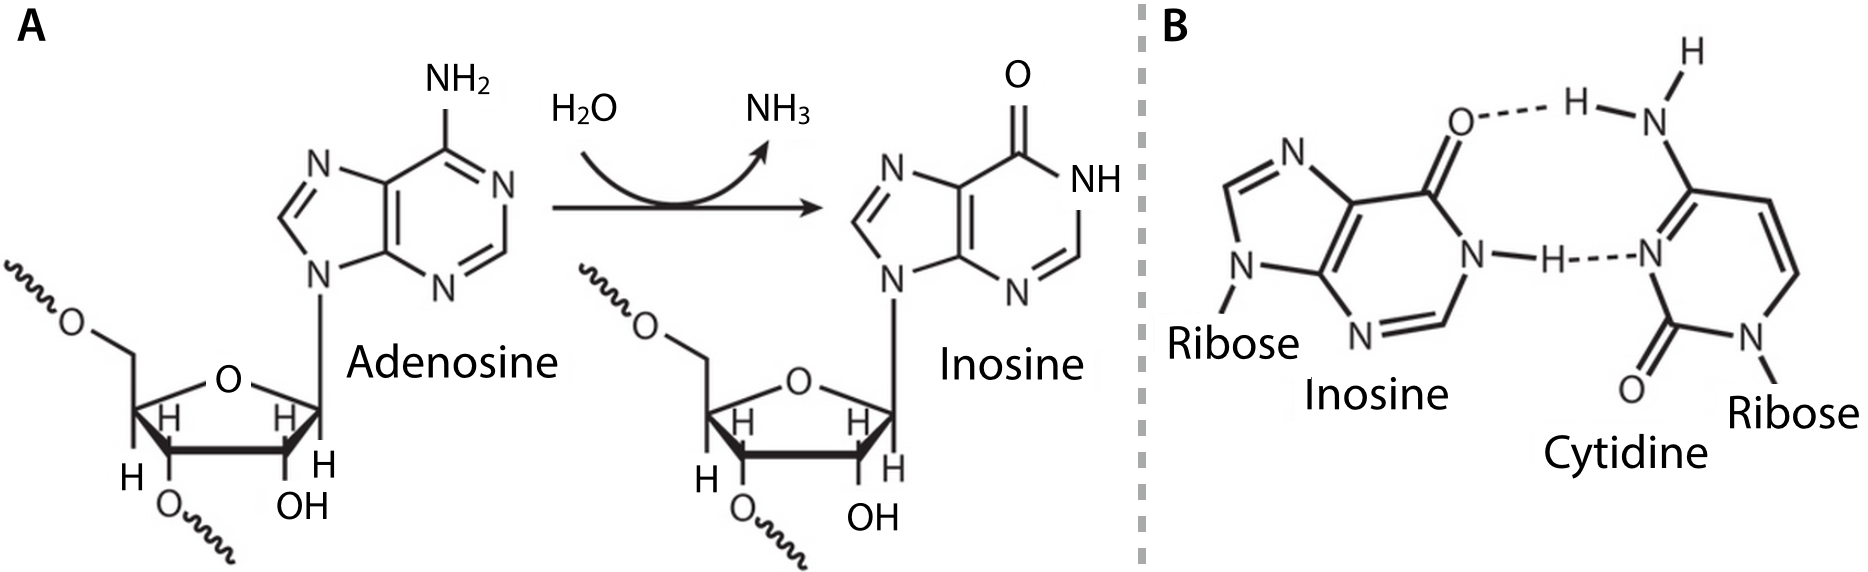
\includegraphics[width=14cm]{Adenosine-inosine.png}
	\end{center}
	\caption{ADARの生化学的な作用機序}
	\begin{flushleft}
		\small{ADARによるアデノシンからイノシンへの化学修飾が触媒される様子を示す。アデノシン塩基はADARによる脱アミノ化反応によってイノシン塩基へと修飾される。}
	\end{flushleft}
	\label{fig:Chemical_reaction}
\end{figure}

Guanosine receptor-2 (GluR2)やSerotonin receptor-2C (5-HTR)など位置特異的なA-to-I editingにおいては、隣接するエクソン-イントロン境界における相補的な配列、ECS (Editing-site complamentary sequence)およびその二次構造の形成が不可欠であることが知られている。加えて、Glutamine receptor (GluR)においては、editingサイト毎にADAR1またはADAR2のどちらか一方に選択的にeditingされることが知られており、位置毎におけるADARの選択性は、ADARの持つdsRBDの数とドメイン間の配列長の相違によるADARと二本鎖RNAとの相互作用が異なることに起因するとの報告がある。図\ref{fig:ADAR}に二本鎖RNAに結合するADARとそのサイトを示した。

\subsection{ADARのドメイン構造}
ADARはA-to-I editingを触媒するdeaminaseドメインと二本鎖RNAに結合するdsRBD (Double-strand binding domain)の2つを共通して有している。dsRBDは65残基程度の長さの中にα-β-β-β-αという特徴的なドメイン構造を持ち、直接的に二本鎖RNAと接触するためA-to-I editingに必須の機能ドメインの一つである。ADAR1においては、Z-DNA-bindingドメインを2つ有しているが、機能的な意味については不明である。ADAR3のみに特徴的にアルギニンリッチな一本鎖RNA結合ドメインのR-domainを持つ。

\begin{figure}[htbp]
	\begin{center}
		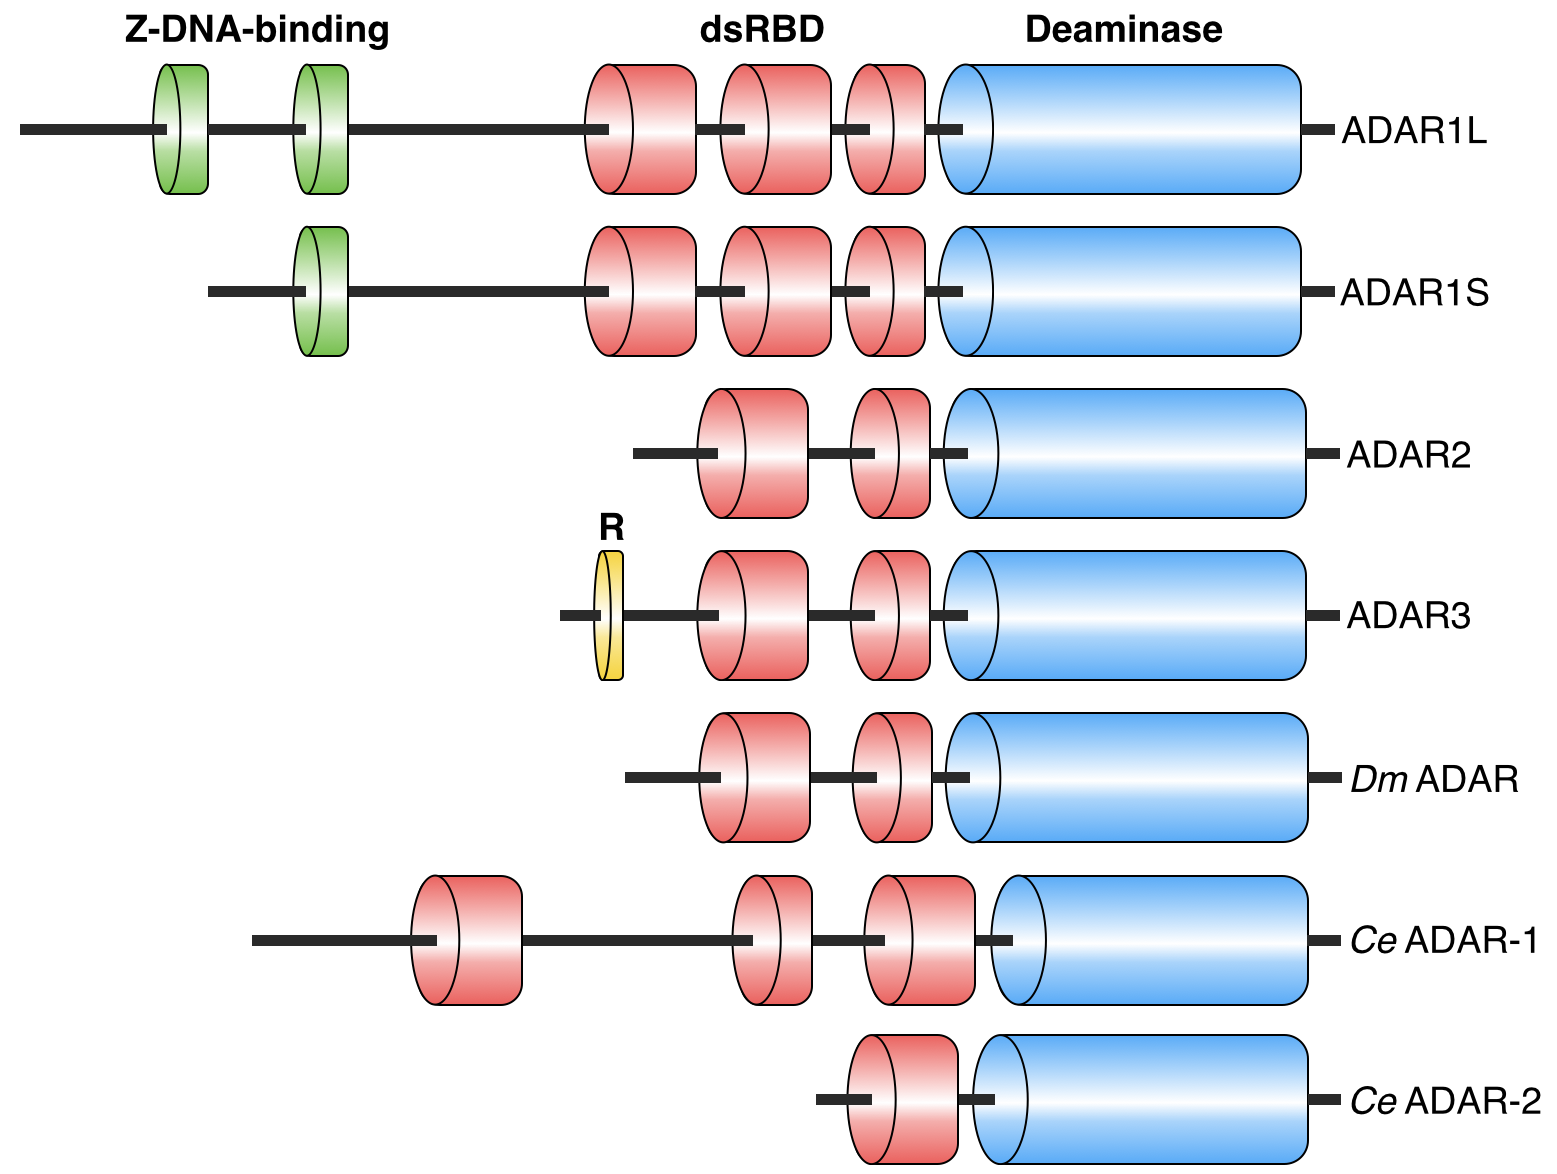
\includegraphics[width=12cm]{Adar_domain.png}
	\end{center}
	\caption{ADARのドメイン構造}
\end{figure}

\subsection{ADARの発現と細胞内局在}
ヒトにおいては、これまでにADAR1、ADAR2、ADAR3の3種類が同定されており、そのうちADAR1については核内および細胞質に局在するADAR1LおよびADAR1Sが知られる他、ADAR3は脳特異的に発現することが知られている。ヒトにおけるADAR1およびADA2は、上記2つの機能ドメインの他にもZ-DNA結合ドメインを有している。
マウス、ショウジョウバエ、線虫におけるADARはバリアントが複数同定されている。

\section{遺伝子領域におけるA-to-I editing}
\subsection{タンパク機能の多様化}

\section{非コード領域におけるA-to-I editing}
\subsection{反復配列におけるA-to-I editing}

\subsection{miRNAへのeditingと遺伝子発現制御}
\begin{figure}[htbp]
	\begin{center}
		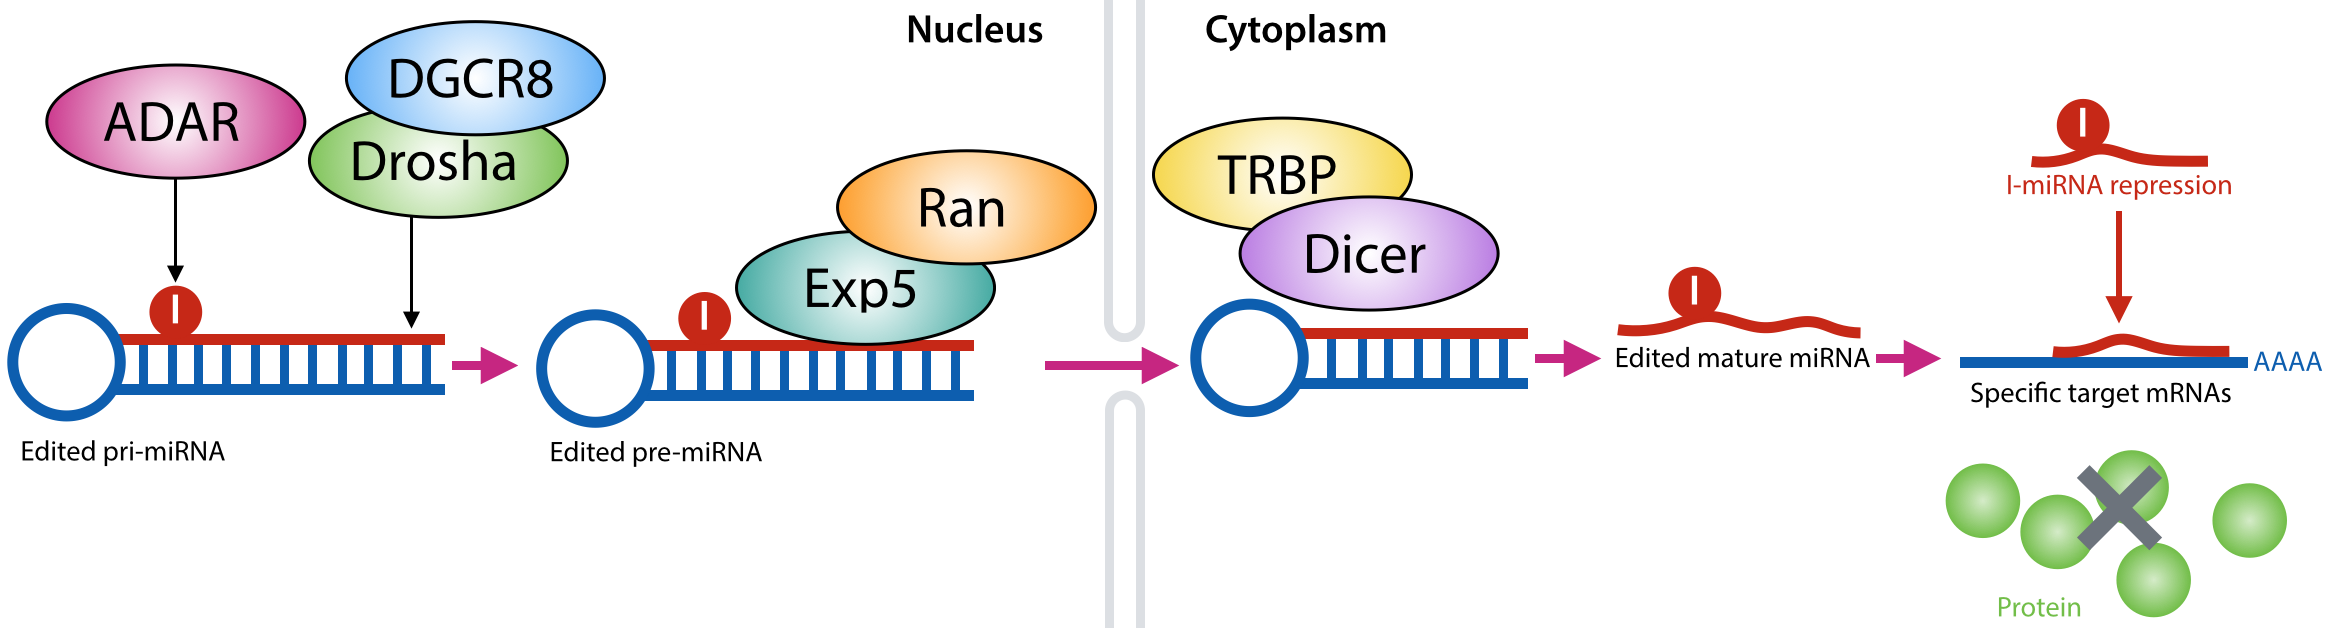
\includegraphics[width=16cm]{miRNA.png}
	\end{center}
	\caption{miRNAへのA-to-I editing}
	\begin{flushleft}
		\small{miRNAの成熟過程においてA-to-I editingを受ける}
	\end{flushleft}
	\label{fig:miRNA}
\end{figure}

\subsection{A-to-I editingとRNAiのクロストーク}
\subsection{A-to-I editingとスプライシングの関係性}

\section{情報学的解析によるRNA editingサイトの検出}
\subsection{超並列シーケンサーによる網羅的解析}
ここ数年、超並列シーケンサーに代表される配列決定技術の躍進的な発展は、多サンプルのゲノムおよびトランスクリプトームのシーケンスを可能にしてきた。RNA editing研究においては、超並列シーケンサーから得られるRNA-seqデータやDNA-seqデータを用いることにより、網羅的で定量性のあるeditingサイトを検出する情報学的手法が精力的に開発されている。超並列シーケンサーから測定されるトランスクリプトームやゲノムの配列情報は、数GBから数百GBの配列データを扱うことになるため、editingサイトの検出は本質的に情報学的な解析が必須となっている。2009年にLiらは、初めてヒトB細胞のRNA-seqデータを用いることにより、10,000箇所を超えるeditingサイトがゲノムワイドに同定されたと報告した。検出された修飾のパタンは、ADARによるA-to-I editing以外にも、A-to-T editingなど未知の修飾の可能性が残されていることを示唆する議論を展開した。また、同定されたeditingサイトは遺伝子間領域にも豊富に分布していること、アミノ酸置換を伴うeditingサイトを新規に同定したと報告した。ところが、この研究が掲載された後、3つの解析結果に対する追従論文が発表され、Liらによる解析結果の95\%以上は擬陽性の可能性があること、解析における擬陽性の原因と排除するための統計的な手法についての提案がされた。

こういったRNA-seqデータを用いることによるゲノムワイドなeditingサイトの分布が明らかになるにつれて、ヒトやマウス、ショウジョウバエといった高等真核生物におけるRNA editingの作用機序、生体内における機能そのものを大きく拡張することになった。
タンパク質の触媒部位へ作用することにより、

\subsection{検出手法の開発}
\subsection{組織およびセルライン特異的なRNA editing}
